\chapter{Related Work}
\label{cha:related-work}

The idea of using electronic devices to foster group interaction in meetings and presentations is not new. Stefik et al. \cite{Stefik:BeyondTheChalkboard} already experimented with the use of personal computers in meeting rooms as early as 1987 and Myers et al. \cite{Myers:CollaborationPDAs} developed a collaboration tool which could be used to annotate PowerPoint slides from PDAs in 1998. Since then, digital whiteboards, telepresence systems, productive multi-user web applications and other computer-aided collaboration tools have become a common sight and we choose to carry smart devices around wherever we go. Surprisingly little research, however, has covered the use of these mobile devices in the context of presentations. Most of these studies were conducted in the educational sector and usually aim at quizzing students, which is why an own sub section is dedicated to classroom related approaches. While most relevant research has concentrated on one aspect, such as real-time polling \cite{Inoue:RealTimeQuestionnaire} or remote-controlling \cite{Chattopadhyay:OfficeSocialRemoteControl}, no system known to us has combined as many interactive mechanisms in one application as ours and allowed seemless integration between them, which sets the present approach apart.

\section{Classroom related}
\label{sec:related-work-classroom}

\begin{figure}
\centering
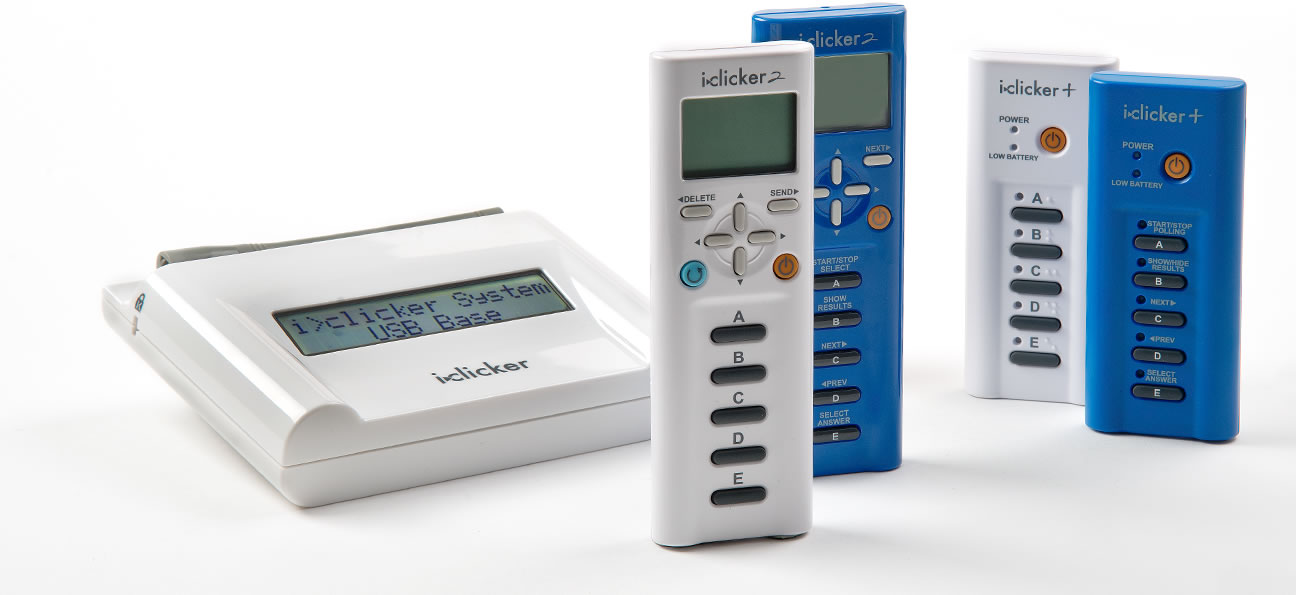
\includegraphics[width=.65\textwidth]{iclickers}
\caption{\emph{i>clicker} devices, used in \cite{Chamillard:StudentResponseSystem}. Image source \cite{iclicker}.}
\label{fig:related-work-iclicker}
\end{figure}

As growing class-sizes have caused student participation to sink drastically \cite{Bry:Backstage}, researchers have tried to deploy mechanisms to make lectures more interactive and engaging. The first ap\-proa\-ches in this field of student-response-systems (SRS) utilised so-called clickers (see figure \ref{fig:related-work-iclicker}) -- remote-control-like devices, connected to a receiver station via radio frequency technology \cite{cuclickers:faq} which can be used for tasks like taking attendance and voting \cite{Chamillard:StudentResponseSystem}. Using these clicker systems has shown to ``yield a strong and positive relationship with student learning'' \cite{Chamillard:StudentResponseSystem}. However, the limitations of clickers -- the need for proprietary hardware and the limited interface consisting only of a few buttons -- lead researchers to experiment with personal mobile devices as input instead. In 2007 Lindquist et al. \cite{Lindquist:ExploringMobilePhonesActiveLearning} presented a system integrated with the University of Washington's Classroom Presenter software, which lets students submit answers to assignments and in-class quizzes via SMS and MMS or using their laptops. Although the mobile phone users struggled with the input of longer messages, they perceived the ubiquity and concenience of using a light-weight personal device as an advantage. Most students, however, were worried about the costs of using SMS or MMS as a requirement in class -- a concern modern devices with internet access and cheap data plans dispel. The first of these web-based approaches were explored around the same time. Esponda \cite{Esponda:ElectronicVotingOnTheFly} for example describes a system in which iPods and other wifi-enabled devices can be used to answer questions during class. What is interesting about her approach is not only the technology used, but also that questions do not have to be prepared in advance, but can also be created on-the-fly, using a pen-based tablet, resulting in more lively and spontaneous student-teacher-interaction.
The creators behind \emph{i>clicker}\footnote{\url{http://www1.iclicker.com/}}, the clicker system used in \cite{Chamillard:StudentResponseSystem}, have also recognised the shortcommings of their hardware-approach and now build mobile apps for students' personal devices. Like\cite{Esponda:ElectronicVotingOnTheFly}, their application makes it possible for lecturers to prepare quizzes beforehands or create polls on-the-fly to monitoring the students' knowledge, understanding and progress. Although also available as iOS and Android app, like most modern approaches, the i>clicker software also has a web version, making use of modern browsers' possibilities and the device-independence of the web as a platform.
The tool \emph{ASQ} \cite{Triglianos:InteractiveWebPresentationsImpress} lets lecturers create HTML5 presentations with \emph{impress.js} \cite{impressjs} which are then distributed to listeners via a link. Students follow the presentations on their mobile devices, and can submit questions connected to the current slide to the speaker. Quizzes (both open questions and multiple-choice) can be embedded in the slides by the teacher. These quizzes can either be graded automatically (for coding assignments and multiple-choice questions), corrected by teaching assistants or by the students in self or peer-assessment. While this project has put a lot of effort into the server-side and administration of slidesets, the present work concentrates more on the client-side and does not provide slide management tools. In contrast to our implementation, however, this approach lacks 
Another interesting approach is presented by Cheng et al. \cite{Cheng:TreebasedOnlinePresentations}, who propose a system which generates HTML presentations from \emph{Microsoft PowerPoint} slides and lets viewers add their own content (either additional material or questions) as vertical sub-slides. This way a tree-like structure is created in which teachers and students collaborate in interactive presentations. This architecture also inspired the sub-slide based presentation space deployed in this software.

Another popular application, with richer audience-spea\-ker-in\-ter\-ac\-tion and an emphasis on listener-listener-interaction is \emph{Backstage} \cite{backstage}. As digital backchannels like Twitter can foster the sense of community within the audience, but are usually hard to follow for presenters, Bry et al.\cite{Bry:Backstage} developed a backchannel specifically for large classrooms. Students can post messages publicly and send private messages to their colleagues. These public posts can be up or down-voted, as well as marked as unrelated. Together with an ageing-algorithm, this community feedback is used to estimate a post's relevance. Important feedback is then presented to the lecturer, to allow him or her to get a better sense for the audiences' opinion and understanding. Additionally, small quizzes and polls serve as performance feedback to the teacher and students. Though one of the most mature systems studied for this thesis, having been developed specifically for classrooms, the use of the software in other scenarios is not ideal. Moreover, most of the features concentrate on listener-listener-interaction, while the present thesis focuses on mechanisms strengthening the speaker-audience-interaction.

Like Backstage, most of these approaches sound promising but are tightly bound to an educational context. The project discussed in this thesis, however aims for a broader field of application and concentrates on business-settings.

\section{Office environments}
\label{sec:related-work-office}

In contrast to classroom-related software, meeting-en\-vi\-ron\-ments usually have an significantly lower amount of participants, as well as a smaller gap between the speaker and the audience. Another difference lies in the polling, surveying and quizzing functionality most of the presented projects offer: while these usually have only one correct answer in educational settings, to grade students \cite{Lindquist:ExploringMobilePhonesActiveLearning, Triglianos:InteractiveWebPresentationsImpress, Bry:Backstage}, the goal in meeting environments is to make decisions and collect ideas, without judgment and often anonymously.
The systems we want to quickly introduce all have a focus on mobile devices and their usage in meetings and office-related presentations and curiously were all developed by Microsoft Research: In \cite{Bohmer:SmartphoneUseRude}, as well as examining the perception of smartphone use in meetings, the mobile application \emph{Meetster} is presented. The study finds that although people primarily use their phones for meeting or work-related tasks, they tend to think their colleagues use theirs for private purposes. Unlike the present thesis, in which mobile devices should be used in the context of presentations, \emph{Meetster} was developed to help getting to know other meeting attendees in a playful way. This changed the perception of using one's smartphone during the meeting and was described as ``fostering social interactions''. While the findings of the study conducted as part of this publication legitimise our approach, this thesis presents a more practical approach, more relevant to the presentation itself, instead of just connecting meeting attendees through a game.

\begin{figure}
\centering\small
\begin{tabular}{cc}
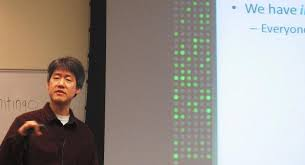
\includegraphics[width=.5\textwidth]{feedback-meetings-ms-research}
 &
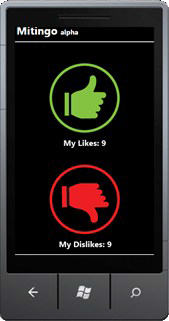
\includegraphics[width=.144\textwidth]{feedback-meetings-ms-research-app} \\
(a) & (b)
\end{tabular}
\caption{\emph{Crowd Feedback} \cite{Teevan:MobileFeedbackDuringPresentation} used during a presentation (a): The bar next to the slides shows one dot per participant in the meeting, the dots can be controlled with the app (b). The feedback dots fade out over time. Image source \cite{Teevan:MobileFeedbackDuringPresentation}.}
\label{fig:related-work-crowd-feedback}
\end{figure}

A system concentrating more on presentations directly is \emph{Crowd Feedback} \cite{Teevan:MobileFeedbackDuringPresentation}, a piece of software which allows listeners to give a speaker continuous, real-time feedback, using their personal devices. A responsive web application with a like and dislike button controls the feedback-system. The participants' reactions are shown with a red (dislike) or green (like) dot for each attendee in a sidebar next to the presentation slides (see figure \ref{fig:related-work-crowd-feedback}). An evaluation of the system showed that the participants felt more engaged with the presentation and connected to other listeners. Many users stated only having the possibility to like or dislike did not reflect enough options and that a button related to the speech pace might have helped. It was also noted that the sidebar was perceived as disturbing and made it harder to pay close attention to the presentation. This study and its conclusions have inspired the implementation of an instant feedback mechanism for listeners in the present work, however, instead of only having the binary like and dislike, the reactions are based on emojis, allowing for more insightful and faceted feedback.

The third study concerns itself with the navigation through slides: \emph{Office Social} \cite{Chattopadhyay:OfficeSocialRemoteControl}, a PowerPoint plugin with companion smartphone app, allows presenters and listeners to navigate through PowerPoint slides using their mobile phones. Members of the audience can either browse the slides privately, or take over the control of the presented slides, allowing them to effictively steer the presentation or discussion. As in the present approach, Chattopadhyay et al.'s software allows members of the audience to review the slides privately, making it possible for latecomers to catch up and to generally estimate the length and direction of the talk \cite{Chattopadhyay:OfficeSocialRemoteControl}. However, as their interface focuses on the navigation between slides, the preview of the slides is fairly small. Our approach tries to focus on the content of the slide and instead of offering big buttons to navigate around, makes use of intuitive swipe gestures, which can potentially be used eye-free more easily \cite{Negulescu:TapSwipeMove}. Another disadvantage is the overhead of having to download a smartphone application before the start of a presentation, as well as the limitation of the application only being available for Windows Phones.

\begin{figure}
\centering
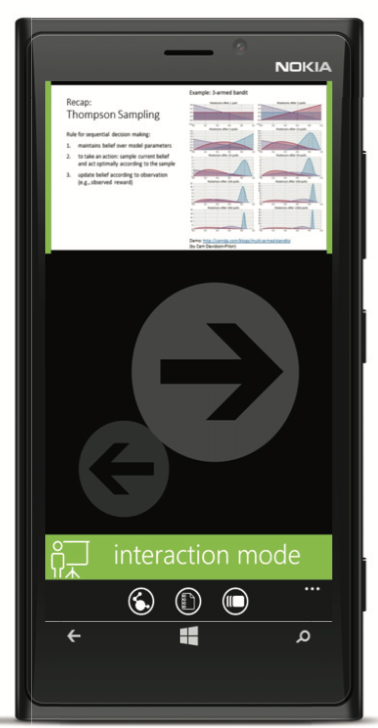
\includegraphics[width=.3\textwidth]{office-social}
\caption{\emph{Office Social} \cite{Chattopadhyay:OfficeSocialRemoteControl}'s smartphone app interface. A preview of the slide is shown on top, followed by big buttons for navigating between slides. In the left picture, the application is in \emph{review} mode, where a local copy of the slides can be navigated through. By pressing a button in the interface the \emph{interaction} mode is activated, allowing listeners to navigate through the master slides (right). Image source \cite{Chattopadhyay:OfficeSocialRemoteControl}.}
\label{fig:related-work-crowd-feedback}
\end{figure}

\section{General presentations}
\label{sec:related-work-general}
Since lectures and meetings both are very specific forms of presentations, a few paragraphs should also be dedicated to general approaches in this third section.
One publication, which concentrates on polls and their real-time evaluation and rendering is \cite{Inoue:RealTimeQuestionnaire}: Inoue et al. present a system which distributes \emph{Microsoft PowerPoint} presentations using modern web-technologies while making it possible to alter and update the slides in presentation mode. This way questionnaires can be answered and their results displayed in real-time. Additionally, members of the audience can add annotations (both handwritten and digital) to slides. Although this approach seems very promising, pictures, videos and other types of media are ignored entirely. Moreover the interface seems too complicated for small devices and is therefore only usable on laptops and maybe tablets.

Two more products, though not subject to scientfic research and more commercial than the approaches presented so far, are \emph{Mentimeter} \cite{mentimeter} and \emph{sli.do} \cite{slido}. Both tools are web applications with real-time polling support, usable in any presentation. Both systems work very similarly: listeners go to the respective website and enter a presentation code to then be connected to the live voting. A handy feature Mentimeter offers is to query the device's location to determine the right presentation. Sli.do on the other hand also supports questions from the audience, which can be up-voted by the listeners, making it easy for speakers and participants in podium-discussions to answer the most relevant questions. Moreover, additionally to multiple-choice polls, sli.do also supports open questions and ratings. While the creators of Mentimeter provide a PowerPoint plugin, sli.do is not directly linked to any presentations. However, the popular canvas-based presentation-tool prezi \cite{prezi}, offers seamless integration with the application. It is worth noting that prezi itself already offers mobile features out of the box: Presentations can be controlled remotely from the speaker's phone or tablet as well as be viewed and followed by members of the audience in real time, using a mobile application.

More web-based presentation tools include \emph{Google Slides} \cite{google-slides} and \emph{PowerPoint Online}\footnote{\url{http://office.live.com/start/PowerPoint.aspx}}. While PowerPoint Online seems to only offer a simplyfied version of the desktop application online, Google Slides also provides mobile features such as editing and authoring slides on phones or tablets and controlling them remotely.

To conclude this chapter, a few words should also be said about the JavaScript presentation library \emph{reveal.js} \cite{revealjs} and its accompanying visual edior \emph{slides} \cite{slides-com}. Reveal.js offers features such as remote controlling slides for the speaker and following presentations on personal devices for members of the audience. However, the installation to achieve the latter so-called \emph{multiplexing} functionality, is fairly complex and involves setting up a socket-io server, running the master-presentation statically and locally and uploading a client version of the presentation to a publicly accessible server. Reveal.js offers a reliable online presentation library and could have served as a starting-point for the project presented in this thesis. However, due to their closed environment, tightly coupled code and lacking support for extensibility, we decided to instead implement an own presentation library (see chapter \ref{cha:implementation}, section \ref{sec:implementation-technologies-unveil}).